\section{Problem (2)}

	Let the mass of the block be $1.7 \ sl$ and the angle $\theta$ be $31^{o}$.

	\begin{figure}[H]
		\begin{center}
			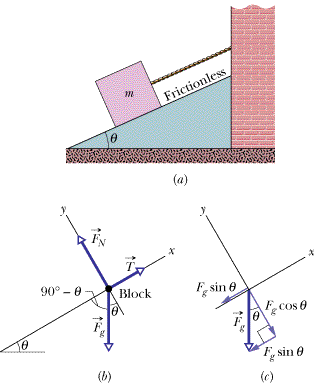
\includegraphics[scale=0.7]{hw5_problem2}
			\caption{Illustration of Problem 2}
			\label{fig:hw5_problem2}
		\end{center}
	\end{figure}

	\subsection{Question (a)}

		Find the tension in the cord:

		\textbf{R:} \newline

		Newton's $2^{nd}$ Law:
		\begin{align}
			\sum F_{x} = \ &ma_{x}& \notag \\
			T - F_{g_{x}} = \ &m(0)& \notag \\
			T = \ &F_{g} \sin 31^{o}& \notag \\
			= \ &(1.7 \ sl)\left( 32.2 \ ft/s^{2} \right)(0.515)& \notag \\
			= \ &28.2 \ sl \times ft/s^{2} = 28.2 \ lb&
		\end{align}

	\subsection{Question (b)}

		Find the normal force acting on the block:

		\textbf{R:} \newline

		Newton's $2^{nd}$ Law:
		\begin{align}
			\sum F_{y} = \ &ma_{y}& \notag \\
			F_{N} - F_{g_{y}} = \ &m(0)& \notag \\
			F_{N} = \ &F_{g} \cos 31^{o}& \notag \\
			= \ &(1.7 \ sl)\left( 32.2 \ ft/s^{2} \right)(0.857)& \notag \\
			= \ &46.9 \ sl \times ft/s^{2} = 46.9 \ lb&
		\end{align}

	\subsection{Question (c)}

		If the cord is cut, find the magnitude of the block's acceleration:

		\textbf{R:} \newline
		\begin{align}
			F_{g_{x}} = \ &28.2 \ lb = ma& \notag \\
			a = \ &\frac{28.2 \ lb}{1.7 \ sl} = 16.6 \ ft/s^{2}&
		\end{align}
